\begin{align}
    &\vec{V}=\myvec{6 & h \\ h & 12} \label{eq:eq1}\\ 
    &\vec{u}=\myvec{11 \\ \frac{31}{2}}  \label{eq:eq2}\\
    & f=20 \label{eq:eq3}
\end{align}
As given in question, the equation represent two straight lines, substitute \eqref{eq:eq1}, \eqref{eq:eq2}, \eqref{eq:eq3} in \eqref{eq:det_1} to satisfy the equation.
\begin{align}
    \mydet{6 & h & 11\\h & 12 & \frac{31}{2}\\11&\frac{31}{2} & 20} = 0 \label{eq:solu_1}
\end{align}
Expanding equation \eqref{eq:solu_1} along row 1 gives
\begin{multline*}
\implies 6\times(240 - \frac{961}{4}) -h\times(20h - \frac{341}{2}) +\\ 11\times(\frac{31h}{2}-132) = 0\\
\end{multline*}
\begin{align}
\implies 20h^{2}-341h+\frac{2907}{2} = 0\\
\implies \boxed{h=\frac{17}{2}} \label{eq:result1}\\
\implies \boxed{h=\frac{171}{20}} \label{eq:result2}
\end{align}
If $h=\frac{17}{2}$ or $h=\frac{171}{20}$, the equation given will represent two straight lines.\\
\\
Sub $h=\frac{17}{2}$ in equation \eqref{eq:question} we get,
\begin{align}
6x^2+17xy+12y^2+22x+31y+20=0 \label{eq:op1}
\end{align}
Equation \eqref{eq:op1} can be expressed as,
\begin{align}
\vec{V}=\vec{V}^T&=\myvec{6 & \frac{17}{2} \\ \frac{17}{2} & 12} \label{eq:eq1vec}\\
\vec{u}&=\myvec{11 \\ \frac{31}{2}} \label{eq:eq2vec}\\
&\vec{f}=20
\end{align}
The pair of straight lines are given by,
\begin{align}
    (\vec{n_1}^{T}\vec{x} - c1)(\vec{n_2}^{T}\vec{x} - c2)=0\label{eq:maineq1}
\end{align}
The slopes of the lines are given by the roots of the polynomial:
\begin{align}
    &cm^2+2bm+a=0 \label{eq:quadr111}\\
    \implies m_i&=\frac{-b\pm{\sqrt{-\det(V)}}}{c}\\
\end{align}
Substituting \eqref{eq:op1} in the equation \eqref{eq:quadr111},
\begin{align}
    &12m^2+17m+6=0 \label{eq:quadr1}\\
    &m_i=\frac{-\frac{17}{2}\pm{\sqrt{\frac{1}{4}}}}{12}\\
    &\implies m_1 = \frac{-2}{3} , m_2 = \frac{-3}{4}\\
    & \vec{m_1}=\myvec{3\\ -2}, \vec{m_2}=\myvec{4\\ -3}\\
    &\implies \vec{n_1}=\myvec{-2\\ -3}, \vec{n_2}=\myvec{-3\\ -4} \label{eq:normal1}
\end{align}
we know that, 
\begin{align}
\vec{n_1}\ast \vec{n_2} = \myvec{a\\2b\\c} \label{eq:conv1}
\end{align}
Convolution of $\vec{n_1}$ and $\vec{n_2}$ can be done by converting $\vec{n_1}$ into a toeplitz matrix and multiplying with $\vec{n_2}$\\
From equation \eqref{eq:normal1}
\begin{align}
    \vec{n_1}=\myvec{-2&0\\-3&-2\\0&-3}
    \vec{n_2}=\myvec{-3\\ -4}\label{eq:conv2}\\
\implies \myvec{-2&0\\-3&-2\\0&-3}\myvec{-3\\ -4} = \myvec{6\\17\\12} = \myvec{a\\2b\\c}\label{eq:conv3}
\end{align}
$\implies$ Equation \eqref{eq:normal1} satisfies \eqref{eq:conv1}\\

$c_1$ and $c_2$ can be obtained as,
\begin{align}
\myvec{\vec{n_1} & \vec{n_2}}\myvec{c_2\\c_1}&=-2\vec{u} \label{eq:aug1}
\end{align}
Substituting \eqref{eq:normal1} in \eqref{eq:aug1}, the augmented matrix is,
\begin{align}
\myvec{-2 & -3 & -22 \\ -3 & -4 & -31}
\xleftrightarrow[R_1\leftarrow \frac{-R_1-3R_2}{2}]{R_2\leftarrow 2R_2-3R_1}
\myvec{1 &0 &5 \\ 0& 1 & 4} \label{eq:aug2}\\
\implies c_1 = 4, c_2=5 \label{eq:const1}
\end{align}
Substituting \eqref{eq:normal1} and \eqref{eq:const1} in \eqref{eq:maineq1} we get,
\begin{multline}
\implies (-2x-3y-4)(3x-4y-5) = 0\\
\implies \boxed{(2x+3y+4)(3x+4y+5) = 0} \label{eq:line1}
\end{multline}
Equation \eqref{eq:line1} represents equations of two straight lines.\\
\renewcommand{\thefigure}{\arabic{figure}}
\begin{figure}[h!]
	\centering
	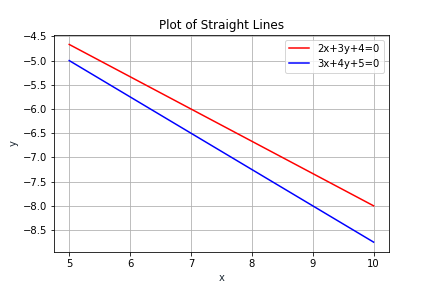
\includegraphics[width=\columnwidth]{./solutions/13/ex2/st1.png}
	\caption{Plot of Straight lines when $h=\frac{17}{2}$}
	\label{myfig}
\end{figure}\\








Similarly, Sub $h=\frac{171}{20}$ in equation \eqref{eq:question} we get,
\begin{align}
20x^2+57xy+40y^2+\frac{220}{3}x+\frac{310}{3}y+\frac{200}{3}=0 \label{eq:op2}
\end{align}

Equation \eqref{eq:op2} can be expressed as,
\begin{align}
\vec{V}=\vec{V}^T&=\myvec{20 & \frac{57}{2} \\ \frac{57}{2} & 40} \label{eq:eq1vec1}\\
\vec{u}&=\myvec{\frac{220}{6} \\ \frac{310}{6}} \label{eq:eq2vec1}\\
&\vec{f}=\frac{200}{3}
\end{align}
The pair of straight lines are given by,
\begin{align}
    (\vec{n_1}^{T}\vec{x} - c1)(\vec{n_2}^{T}\vec{x} - c2)=0\label{eq:maineq2}
\end{align}
Substituting \eqref{eq:op2} in the equation \eqref{eq:quadr111},
\begin{align}
    &40m^2+57m+20=0 \label{eq:quadr11}\\
    &m_i=\frac{-\frac{57}{2}\pm{\sqrt{\frac{49}{4}}}}{40}\\
    &\implies m_1 = \frac{-5}{8} , m_2 = \frac{-4}{5}\\
    & \vec{m_1}=\myvec{8\\ -5}, \vec{m_2}=\myvec{5\\ -4}\\
    &\implies \vec{n_1}=\myvec{-5\\ -8}, \vec{n_2}=\myvec{-4\\ -5} \label{eq:normal11}
\end{align}
Convolution of $\vec{n_1}$ and $\vec{n_2}$ can be done by converting $\vec{n_1}$ into a toeplitz matrix and multiplying with $\vec{n_2}$\\
From equation \eqref{eq:normal11}
\begin{align}
    \vec{n_1}=\myvec{-5&0\\-8&-5\\0&-8}
    \vec{n_2}=\myvec{-4\\ -5}\label{eq:conv21}\\
\implies \myvec{-5&0\\-8&-5\\0&-8}\myvec{-4\\ -5} = \myvec{20\\57\\40} = \myvec{a\\2b\\c}\label{eq:conv31}
\end{align}
$\implies$ Equation \eqref{eq:normal11} satisfies \eqref{eq:conv1}\\

$c_1$ and $c_2$ can be obtained as,
\begin{align}
\myvec{\vec{n_1} & \vec{n_2}}\myvec{c_2\\c_1}&=-2\vec{u} \label{eq:aug11}
\end{align}
Substituting \eqref{eq:normal11} in \eqref{eq:aug11}, the augmented matrix is,
\begin{align}
\myvec{-5 & -4 & -\frac{220}{3} \\ -8 & -5 & -\frac{310}{3}}
\xleftrightarrow[R_1\leftarrow \frac{-R_1-4R_2}{5}]{R_2\leftarrow \frac{5R_2-8R_1}{7}}
\myvec{1 &0 &\frac{20}{3} \\ 0& 1 & 10} \label{eq:aug21}\\
\implies c_1 = 10, c_2=\frac{20}{3} \label{eq:const11}
\end{align}

Substituting \eqref{eq:normal11} and \eqref{eq:const11} in \eqref{eq:maineq2} we get,
\begin{multline}
\implies \boxed{(5x+8y+10)(4x+5y+\frac{20}{3}) = 0} \label{eq:line2}
\end{multline}
Equation \eqref{eq:line2} represents equations of two straight lines.
\renewcommand{\thefigure}{\arabic{figure}}
\begin{figure}[h!]
	\centering
	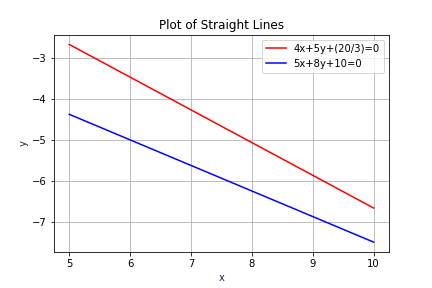
\includegraphics[width=\columnwidth]{./solutions/13/ex2/st2.png}
	\caption{Plot of Straight lines when $h=\frac{171}{20}$}
	\label{myfig}
\end{figure}
